\documentclass[12pt, a4paper, twoside]{report}

\usepackage[spanish]{babel}
\decimalpoint
\usepackage[utf8x]{inputenc}
\usepackage[T1]{fontenc}

% Para usar fuentes de letra distintas a la que viene por defecto es probable que te pida usar un compilador diferente a pdflatex, se puede cambiar fácilmente en el menú arriba a la izquierda.

%\usepackage{fontspec}
%\setmainfont{Arial}
\usepackage[table,xcdraw]{xcolor}
\usepackage{listings}

\usepackage{minted}
\usemintedstyle{pastie}

\usepackage{tikz}
\usepackage{pgfplots}
\pgfplotsset{compat=1.17}

\usepackage{filecontents}

\usepackage{wrapfig}

\usepackage{csquotes}
\usepackage{epigraph}
\usepackage[font={footnotesize, sf}]{caption}
\usepackage{shadethm}
\usepackage{hyperref}
\hypersetup{hypertexnames=false, colorlinks=true, urlcolor=blue, linkcolor=black, citecolor=blue}
\usepackage{lscape}
\usepackage{subcaption}
\usepackage{amsmath}
\usepackage{graphicx}
\usepackage[colorinlistoftodos]{todonotes}
\usepackage[final]{pdfpages}
\usepackage[all]{nowidow}
\usepackage{multicol}
\usepackage{booktabs}
\usepackage{multirow}

\usepackage[]{algorithm2e}

\usepackage{titlesec}

\titleformat{\chapter}[block]
  {\scshape\huge}{\thechapter.}{1em}{\Huge}
\titlespacing*{\chapter}{0pt}{-19pt}{40pt}

\definecolor{graybox}{RGB}{235, 235, 235}
\newcommand{\jesitt}[1]{\colorbox{graybox}{\textcolor{red}{\texttt{#1}}}}

\renewcommand{\baselinestretch}{1.2}
\setlength{\parskip}{1em}
\renewcommand{\mkbegdispquote}[2]{\itshape}

\newshadetheorem{thm}{Comentario}
\definecolor{shadethmcolor}{HTML}{EDF8FF}
\definecolor{shaderulecolor}{HTML}{45CFFF}
\fontfamily{ttfamily}
\setlength{\shadeboxrule}{.4pt}


%% Sets page size and margins
\usepackage[a4paper,top=2.5cm,bottom=2.5cm,left=2.5cm,right=2.5cm,marginparwidth=1.75cm]{geometry}

%Options: Sonny, Lenny, Glenn, Conny, Rejne, Bjarne, Bjornstrup
% \usepackage[Sonny]{fncychap}

\title{Análisis de textos médicos \\mediante NLP}
\author{Jesús Enrique Cartas Rascón}
% Puedes cambiar el profesor, la asignatura y demás en el archivo title/title.tex

\begin{document}
\begin{titlepage}

\newcommand{\HRule}{\rule{\linewidth}{0.5mm}} % Defines a new command for the horizontal lines, change thickness here

\center % Center everything on the page

%----------------------------------------------------------------------------------------
%	HEADING SECTIONS
%----------------------------------------------------------------------------------------
\quad\\[1.5cm]
%\textsc{\LARGE MSc Thesis}\\[1.5cm] % Name of your university/college
\textsc{\Large Trabajo Fin de Máster}\\[0.5cm] % Major heading such as course name

%----------------------------------------------------------------------------------------
%	TITLE SECTION
%----------------------------------------------------------------------------------------
\makeatletter
\HRule \\[0.4cm]
{ \huge \bfseries \@title}\\[0.4cm] % Title of your document
\HRule \\[1.5cm]
 
%----------------------------------------------------------------------------------------
%	AUTHOR SECTION
%----------------------------------------------------------------------------------------

\begin{minipage}{0.4\textwidth}
\begin{flushleft} \large
\emph{Autor:}\\
\@author % Your name
\end{flushleft}
\end{minipage}
~
\begin{minipage}{0.4\textwidth}
\begin{flushright} \large
\emph{Profesor:} \\
Rocío Romero Zaliz
% Uncomment the following lines if there's a co-supervisor
%\\[1.2em] % Supervisor's Name
%\emph{Co-Supervisor:} \\
%Dr. Adam Smith % second marker's name
\end{flushright}
\end{minipage}\\[3cm]
\makeatother


%----------------------------------------------------------------------------------------
%	DATE SECTION
%----------------------------------------------------------------------------------------

\vfill % Fill the rest of the page with whitespace

\end{titlepage}

\begin{abstract}
  En el ámbito de la medicina se almacena una gran cantidad de información relevante: desde valores numéricos correspondientes a signos vitales hasta texto plano que realiza un especialista para completar un informe. Muchas veces los datos guardados en el historial médico de un paciente, que no tiene una estructura determinada, son ignorados. Este proyecto propone recuperar texto médico sin formato utilizando técnicas de Procesamiento del Lenguaje Natural y modelos generativos de lenguaje, para extraer nuevo conocimiento que pueda utilizarse para complementar la información estructurada y mejorar en la clasificación y tratamiento de los pacientes.

\begin{center}
  \textbf{Abstract}
\end{center}


  Medical reports hold very important information, ranging from numerical and categorical values to plain text written by the professional in charge. These exerpts are often ignored because of their unstructured nature. This project aims to focus on these pieces of text, using Natural Language Processing techniques, as well as generative language models, in order to recover the information and knowledge they hold, and present them in an easier to interpret, easier to index way. This process ultimately will create new structured data that will complement and enrich the original report, allowing for better patient treatment and data management.

\end{abstract}


% Descomentar aquellos que sean necesarios
\tableofcontents
\listoffigures
%\listoftables
%\listoflistings



% Contenido del documento
\chapter{Introducción}

En este capítulo introduciremos los principales problemas existentes en el contexto de minería de datos en el texto médico y pronpodremos una solución que se desarrollará a lo largo del documento.

\section{Texto sin formato}
Toda atención médica dispone de documentos que recogen toda la información relacionada con el paciente, enfermedad, y un seguimiento de ambos, así como los recursos a utilizar. En estos documentos suele haber una sección en la que el o la profesional en cuestión describe, en lo que podríamos denominar \textit{texto sin formato} todas estos factores. Debido a la carencia de formato, es difícil trabajar con dichas secciones, por lo que se suelen ignorar.

La idea es centrar nuestra atención en esas secciones de texto, con objeto de obtener la mayor cantidad de información posible y anexarla, ahora con formato, al documento del que provienen, enriqueciendo el informe y habilitando nuevas claves de búsqueda, así como mejorando el indexado de los documentos.


\section{Falta de datos}
Uno de los principales problemas a los que nos enfrentamos es la falta de \textit{datasets} o conjuntos de datos en los que estos documentos estén presentes. 

Se buscarán y agregarán tantas fuentes de datos como sea posible, se unificarán y se creará una herramienta que aproveche todos los datos disponibles públicamente para generar datos nuevos.

\section{Objetivos}
Dado este marco, describiremos en esta sección los objetivos de nuestro trabajo.

En primer lugar, se agregarán todas las fuentes de información públicas que nos provean con datos de comentarios médicos listos para su minería y análisis.

Utilizando todos estos datos, se hará una evaluación de las herramientas que ya existen en el estado del arte. Haremos una revisión de cómo se utilizan y del rendimiento de dichas herramientas. 

Sin embargo, para evaluar dichas herramientas, no utilizaremos los datos encontrados, sino que efectuaremos un flujo de trabajo alternativo. Utilizando técnicas de aprendizaje automático y generativo, crearemos un modelo que sea capaz de generar tantos comentarios médicos como sea necesario. La idea es suplir la carencia de datos con un modelo generativo, de forma que no se tenga que lidiar con aspectos de privacidad o licencia, ya que todos los comentarios serían generados de forma sintética. 

Si bien los comentarios son sintéticos, deben ser lo suficientemente convincentes como para que la evaluación de las herramientas sea fiel y rigurosa. Esto ofrece una herramienta para los desarrolladores de las herramientas que habilita a un mejor y más fructífero desarrollo, ya que se disponde de una cantidad, \textit{idealmente infinita} de comentarios.





\chapter{Fundamentos de la minería de texto}
En este capítulo discutiremos algunas de las técnicas y términos más importantes a la hora de hablar de minería de texto, así como minería de datos en general, con objeto de que todas las consideraciones realizadas posteriormente queden claras.

En \textit{Text Mining Applied to Electronic Medical Records: A Literature Review}~\cite{textmining2015} se hace una revisión de los diferentes aspectos a tener en cuenta durante el procesamiento de textos médicos. Nos apoyaremos en gran medida en la estructura, contenidos y referencias de este artículo, que resume muy bien todo lo que necesitamos saber para resolver nuestro problema.

\section{Minería de datos}
La minería de datos es una rama de la informática que se dedica a encontrar tendencias y patrones en grandes volúmenes de información. Estas tendencias y patrones crean \textit{conocimiento} a partir de los datos, es decir: información estructurada desde los datos no estructurados. Esta información es muy valiosa y contribuye en las decisiones que se vayan a tomar o a monitorizar algunos aspectos que sean de vital importancia para el interesado. 

La minería de datos puede dividirse en un número de técnicas que funcionan de forma diferente en función del tipo de datos que tengamos y la información que busquemos.

\begin{enumerate}
    \item \textbf{Asociación}: esta técnica se centra en encontrar relaciones entre las distintas variables de nuestros datos, con objeto de encontrar muestras que sean estadísticamente dependientes. Una de las técnicas más utilizadas son las reglas de asociación, cuya salida tras el cálculo son un conjunto de reglas con antecedentes y consecuentes, muy fácilmente interpretables por cualquier persona, familiarizada o no con la ciencia de datos. \cite{associationrules1991}
    \item \textbf{Clasificación}: el proceso de clasificación trata de asignar una categoría a un conjunto de elementos que tengan algún aspecto en común. La clasificación en la minería de datos es una de las técnicas más utilizadas, ya que la naturaleza de gran parte de los datos responden bien a este método. \cite{Kumar2012ClassificationAF}
    \item \textbf{Agrupamiento}: también denominado \textit{clustering} trata de agrupar muestras que tengan características similares. A diferencia de la clasificación, aquí no tenemos una etiqueta o categoría a la que asignar las muestras, sino que las agrupamos \textit{a ciegas}, simplemente basándonos en alguna métrica para evaluar la distancia que haya entre un determinado par de muestras. \cite{Jain1999DataCA}
    \item \textbf{Predicción}: la predicción nos ayuda a encontrar tendencias entre variables, generalmente en datos con una componente temporal fuerte. \cite{han2012mining} Es común poder predecir si un paciente sufrirá una determinada enfermedad conociendo su historial médico, por ejemplo.
    \item \textbf{Identificación de patrones secuenciales}: Al igual que la predicción, se trabaja sobre datos con una componente temporal marcada. En este caso, se buscan patrones, es decir, conjuntos o cadenas de muestras que aparecen de forma frecuente en un orden concreto.
\end{enumerate}


\section{Minería de texto}
En esta sección, discutiremos los diferentes aspectos a tener en cuenta en la minería de textos en concreto, tras haber abordado el concepto de minería de datos en un ámbito más general.


\subsection{Términos}
Definiremos algunos de los términos más utilizados en esta disciplina, guiándonos principalmente por el trabajo de Kamran Kowsari, \textit{Text Classification Algorithms: A Survey}~\cite{Kowsari2019TextCA}.

\subsubsection{Tokens}
\label{sec:tokens}
El término más esencial en minería de textos es \textit{token}. Un token es la mínima unidad en la que dividiremos un cuerpo de texto a la hora de analizarlo. Este elemento suele corresponderse con una palabra, que en el contexto de la mayoría de los idiomas corresponde con un conjunto de letras separado por espacios anterior y posteriormente. Esto da lugar a la creación de \textit{Tokenizers}, algoritmos que toman un cuerpo de texto como una cadena de caracteres muy larga, y devuelven un vector de palabras. Estos \textit{tokenizers } no han de tomar el espacio en blanco necesariamente ni exclusivamente como criterio divisor, aunque suele ser lo más común. Algunos de los \textit{tokenizers} más famosos son:

\begin{itemize}
    
    \item \textbf{Tokenizers de palabras}
    \begin{itemize}
        \item \textbf{Standard Tokenizer}: El Standard Tokenizer divide el texto en términos siguiendo los límites de las palabras según están definidos en el algoritmo \textit{Unicode Text Segmentation}. 
        \item \textbf{Letter Tokenizer}: Divide el texto en términos cada vez que encuentra un carácter que no es una letra.
        \item \textbf{Whitespace Tokenizer}: Toma como criterio divisor el espacio en blanco.
        \item \textbf{Language Tokenizer}: Otros tipos de tokenizers adaptados a diferentes idiomas, como el inglés, que es el idioma más estudiado con diferencia, pero también otros idiomas con caracteres y reglas diferentes a aquellos basados en reglas occidentales, como el tailandés o el chino.
    \end{itemize}
    \item \textbf{Tokenizers de palabras parciales}
    \begin{itemize}
        \item \textbf{N-Gram Tokenizer}: Este tokenizador incluye un parámetro adicional. Primero divide el texto con alguna de las reglas mencionadas anteriormente, y posteriormente, divide cada término del vector resultante en una ventana deslizante de $n$ elementos, (de ahí \textit{N-Gram}). Por ejemplo: \textit{quick fox} devolvería $[$qu, ui, ic, ck$]$, $[$fo, ox$]$, dado un $n = 2$. Estos tokenizers también pueden utilizarse a nivel de párrafo, por lo que se devolverían pares de palabras, algo que puede ser muy útil para el análisis de \textit{dichos} o expresiones.
    \end{itemize}
    \item \textbf{Tokenizers de texto estructurado}
    \begin{itemize}
        \item \textbf{Pattern Tokenizer}: este tokenizer utiliza el patrón provisto como parámetro para la división de texto, utilizando expresiones regulares.
        \item \textbf{Simple Pattern Tokenizer}: este tokenizer utiliza el patrón provisto como parámetro para la división de texto, utilizando expresiones optimizadas para el patrón dado, lo que hace que funcione generalmente más rápido pero también será más específico.
    \end{itemize}
\end{itemize}

En resumen, un tokenizer es un algoritmo que divide el texto provisto siguiendo los criterios definidos por el usuario, devolviendo un vector con los elementos del texto divididos atendiendo a dichos criterios. Es una de las herramientas esenciales en la minería de texto, ya que permite generar la mínima unidad de información a partir de la que se extraerá conocimiento.

\subsubsection{Palabras vacías}
\label{sec:stopwords}
Las palabras vacías o \textit{stopwords} son términos presentes en un idioma que sirven de apoyo para la formulación de oraciones pero que no poseen información en sí. Nos referimos a los artículos, determinantes, preposiciones, etc.

Estos términos son considerados como \textit{ruido} en el procesamiento de texto, por lo que lo más usual es disponer de un diccionario de términos vacíos y filtrar el texto original, eliminando dichos términos. De esta forma, nos quedamos con las palabras más importantes. Los símbolos de puntuación también se suelen considerar como ruido; si bien son esenciales para la comprensión y estructuración de texto para los humanos, suponen un detrimento para algoritmos de clasificación.

Sin embargo, esta operación es delicada y no siempre ofrecerá buenos resultados. Por ejemplo, si tratamos de inferir la intención de la oración \textit{No me gusta el fútbol} y pasamos previamente un filtro de palabras vacías, el texto resultante sería \textit{gusta fútbol}. Dados estos términos, se infiere que se está opinando de forma positiva acerca del tema \textit{fútbol}, cuando no es así.

Este caso particular está descrito en la literatura como \textit{negation handling}, en trabajos como \cite{Farooq2017NegationHI} o \cite{Ali2020ConventionalAS}. Aún así, hay muchos factores que se deben tener en cuenta antes de eliminar términos de una oración.



\subsubsection{Stemming y Lematización}
Stemming hace referencia a la gestión de palabras con prefijos o sufijos para su integración en una frase, como plurales (casa, casa\textbf{s}). Se trata de eliminar los posibles complementos añadidos con objeto de normalizar las palabras y que todas tengan la misma forma. En este caso también han de tenerse en cuenta las negaciones (típico, \textbf{a}típico).

La lematización va un paso más allá y trata de encontrar la raíz de las palabras, obteniendo una normalización más estricta. Un buen ejemplo son la conjugación de los verbos: de \textit{estudiando}, \textit{estudiante} o \textit{estudio} obtenemos \textit{estudi-}. \cite{Lemmatization2014} 


\subsubsection{Frecuencias: TF, IDF}
\label{sec:tfidf}
Uno de los datos más importantes a obtener de un texto es la frecuencia de palabras. Esta operación es tan simple como suena: contar cuántas veces aparece cada palabra y anotarlo en una estructura similar a un diccionario. Este término se conoce como \textit{Term Frequency} o TF. Estos valores suelen representarse en una escala logarítmica, con objeto de que las palabras muy dominantes no eclipsen a las menos frecuentes.

Del campo de teoría de la información \cite{information2001} conocemos que aquellos términos que aparezcan con una frecuencia muy alta poseerán menos información que aquellos que aparezcan menos. Como vimos en la sección \ref{sec:stopwords}, eliminamos las palabras vacías porque aparecían mucho. Es decir, un artículo como \textit{el} o una preposición como \textit{de} tendrían una frecuencia desproporcionada, cuando en realidad no aportan ninguna información. 


De forma similar, el valor \textit{Inverse Document Frequency}~\cite{Jones2004ASI} trata de abarcar esta frecuencia pero en un conjunto de documentos, añadiendo la inversa de la frecuencia por documento. Esta métrica se utiliza mucho en conjunción con la TF, resultando en la TF-IDF, que trata de medir la relevancia de un término en un conjunto de documentos. Esto resulta en el cálculo:

\begin{equation}
    W(d, t) = TF(d, t) * log(\frac{N}{df(t)})
\end{equation}

donde $d$ es un documento del conjunto de documentos con cardinalidad $N$, $t$ es el término en concreto y $df(t)$ es el número de documentos que contienen el término $t$.


\subsubsection{Bolsas de palabras}
Conociendo el concepto de frecuencias de palabaras, una de las aplicaciones directas son las bolsas de palabras, que recogen en una estructura con forma de diccionario cada término y su frecuencia.

De esta forma, tenemos un \textit{ranking} para cada término. Esto se utiliza extensivamente en sistemas de recomendación, en donde una consulta provista por un usuario se compara con la bolsa de palabras del posible conjunto de documentos, y este conjunto va afinándose conforme se van comparando los conjuntos de palabras. El resultado es una búsqueda más refinada que devuelve documentos más relevantes con respecto a la consulta realizada.

\subsubsection{Word Clouds}
Las nubes de palabras o \textit{Word Clouds} son un tipo de visualización especializada en conjuntos de datos de texto. Consisten en representar el conjunto de palabras más relevantes del texto que analicemos, disponiendo dicho conjunto de forma distrubida por la imagen. Por lo general, se suelen utilizar códigos de color o tamaño para aludir a factores como la frecuencia o la relevancia de dicha palabra en el texto.

Dada una bolsa de palabras, podemos tomar los $n$ términos más presentes y escribirlos en una imagen, haciendo la fuente tanto más grande cuanto más aparezca dicha palabra. Esto ofrece una manera rápida e intuitiva de averiguar el tema del cuerpo del texto y sus términos más relevantes.


\subsection{Técnicas}
En esta sección discutiremos algunas de las técnicas avanzadas más utilizadas en procesamiento y análisis de texto que además utilizaremos en nuestra implementación directa o indirectamente.

\subsubsection{\textit{Word Embeddings}}
Esta técnica esencialmente trata de convertir los diferentes términos en vectores de números reales, ya que esto los convierte en objetos matemáticos fáciles de comparar y procesar. Matemáticamente hablando corresponde con una representación de un espacio $n$-dimensional a un espacio vectorial continuo de menor tamaño, donde $n$ es el número total de términos presentes en todos los documentos.

Esta técnica ha sido estudiada en profundidad en varios proyectos:

\begin{itemize}
    \item \textbf{Word2Vec}: esta técnica trata de representar las palabras como vectores utilizando una red neuronal con dos capas, haciendo uso de una bolsa de palabras continua (CBOW) y el modelo del Skip Gram. \cite{Mikolov2013Word2Vec}
    \item \textbf{GloVe}: acrónimo de \textit{Global Vectors for Word Representation}, es una técnica muy similar a la \textit{Word2Vec}, con la particularidad de estar preentrenada en grandes corpus de texto, basados en Wikipedia y Gigaword. \cite{Pennington2014GloveGV}
    \item \textbf{FastText}: es una técnica desarrollada por Facebook. Esta técnica hace uso de la técnica de los $n$-grams para su entrenamiento, obteniendo una representación de los términos mucho más granular. \cite{Bojanowski2017EnrichingWV}
    \item \textbf{Contextualized Word Representations}: esta técnica hace uso del contexto de las palabras para tratar de encontrar una representación y relación entre ellas. Esta técnica basa su funcionamiento en el uso de Long-Short Term Memory, un tipo de red neuronal recurrente muy utilizada en procesamiento de texto, en la que ahondaremos más en profundidad en secciones posteriores de este documento. \cite{Melamud2016context2vecLG}
\end{itemize}

\subsubsection{Reducción de dimensionalidad}
La reducción de dimensionalidad es una técnica que permite proyectar el espacio en el que se hallan nuestros datos en un subespacio de menor dimensionalidad, con objeto de facilitar el cálculo de las propiedades de dichos datos sin tener que utilizar todas sus características. Es común encontrar conjuntos de datos con un número de dimensiones muy alto, que hace inviable su estudio.

Las principales técnicas desarrolladas para reducir la dimensionalidad incluyen:

\begin{itemize}
    \item \textbf{Principal Component Analysis (PCA)}: PCA o análisis de componentes principales trata de encontrar un subespacio latente que represente a los datos encontrando aquellas variables que estén menos relacionadas y que maximicen la varianza, para conservar la mayor cantidad de variabilidad posible. \cite{Jolliffe:1986} 
    \item \textbf{Independent Component Analysis (ICA)}: es una técnica similar que trata de expresar los datos con transformaciones lineales. \cite{Hyvrinen2014TopographicIC}
    \item \textbf{Linear Discriminant Analysis (LDA)}: es otro método muy utilizado cuando los datos son de caracter categórico y no tienen una proporcion uniforme intraclase. \cite{LDA2009}
\end{itemize}

Toda esta familia de algoritmos resulta muy conveniente para \textit{comprimir} datos de alta dimensionalidad y extraer solo las \textbf{características principales} de los mismos. Se suelen usar en etapas de preprocesamiento, donde los datos resultantes se pasan a los algoritmos a entrenar, consiguiendo un mejor resultado y rendimiento en comparación con los datos sin preprocesar.

\subsubsection{Clasificación de texto}
Por último, abordaremos las principales técnicas para clasficar texto, ámbito importante en nuestro proyecto, así como una breve explicación de las mismas. Al igual que en las secciones anteriores, no es nuestro objetivo estudiarlas en profundida, pero más bien ofrecer una vista general del panorama en cuanto a esta tecnología con objeto de que el lector se familiarice con los términos.


Los principales algoritmos de clasificación de texto, entre otros, son los siguientes:

\begin{itemize}
    \item \textbf{Boosting y bagging}: boosting y bagging son dos métodos basados en lo que se denomina en la literatura como \textit{ensemble learning}. Estos métodos no son algoritmos de clasificación en sí, sino que son métodos aplicables a cualquier modelo. Esta técnica utiliza un gran número de modelos que funcionan muy bien para casos muy específicos pero no generalizan correctamente. La idea es que la respuesta conjunta de todos los modelos provea la respuesta correcta de forma más probable. \cite{Bauer2004AnEC}
    
    \item \textbf{Naïve Bayes}: estos modelos utilizan el poder de inferencia del cálculo de probabilidades condicionales para la categorización, más en concreto, la categorización de texto. Esta familia de modelos se ha demostrado que funcionan particularmente bien para esta tarea, además de ser muy rápidos. \cite{FrankNaive2006}

    \item \textbf{Regresión logística}: la regresión logística es uno de los métodos de aprendizaje más simples, junto con la regresión linear. La regresión logística es una especialización de la regresión lineal, de forma que se utiliza una función logística para predecir categorías discretas, no continuas. \cite{logitText}

    \item \textbf{Redes neuronales recurrentes}: las redes neuronales recurrentes son una especialización de las redes neuronales en las que un subonjunto de las neuronas reciben su salida como una entrada, generándose ciclos de retroalimentación o \textit{feedback}. Estas redes funcionan especialmente bien con datos con patrones y componentes temporales, características especialmente destacables del lenguaje humano, así como de la música o vídeo. \cite{ZhouLSTM}

    \item \textbf{Máquinas de Soporte Vectorial}: Las Support Vector Machines (SVM) son modelos muy conocidos de aprendizaje supervisado para clasificación y regresión. Aunque originalmente se concibieron como modelos de separación lineal entre las clases a clasificar, se pueden modificar sus \textit{kernels} para obtener clasificadores no lineales. El funcionamiento de estos modelos en clasificación de texto es muy bueno como se sugiere en \cite{SVMJoa1998}.
\end{itemize}


Existen otras técnicas en clasificación de texto, como \textit{K Nearest Neighbours}~\cite{KNNXiao2007}, árboles de decisión~\cite{DecisionTreeNoorman2018} o \textit{Random Forests}~\cite{breiman2001random}, entre muchas otras. 

\section{Estado del arte}

Por último, hablaremos de los diferentes lenguajes y vocabularios médicos disponibles en el estado del arte que ayudan a extraer conocimiento de la terminología médica.

Además, mencionaremos brevemente los tres proyectos más grandes de lenguaje generativo hasta la fecha, con objeto de entender qué es lo que hacen para poder integrar dichas técnicas en nuestro modelo.

\subsection{Terminología médica}

Debido al vocabulario y términos tan específicos con los que se tratan en el ámbito de la medicina, si deseamos automatizar cualquier proceso de extracción de conocimento debemos tener en cuenta este factor. Es por ello que en 1999 se creó el Systemized Nomenclature of Medicine -– Clinical Terms (SNOMED). 

El SNOMED es una colección de términos sistemáticamente organizada, que provee códigos, términos, sinónimos y definiciones utilizadas en el ámbito de la medicina.

A raíz del SNOMED aparecen vocabularios más específicos que matizan aspectos que pudieran no haberse considerado en el sistema inicial. Todas estas colecciones se aglomeran en el Unified Medical Language System (UMLS), que incluye al SNOMED.

Estos vocabularios son de vital importancia para modelos de lenguaje médico, ya que proveen un sistema rápido y accesible para el etiquetado y clasificación, resumen o extracción de palabras clave de extractos médicos o similares. Los \textbf{reconocedores de entidades} hacen un especial uso de este sistema, como veremos en capítulos posteriores.



\subsection{Transformers}
En esta sección hablaremos del Transformer, un tipo de arquitectura de red neuronal creada por ingenieros de Google \cite{TransformerAshish2017}, en más profundidad, sus características principales en contraste con las demás tecnologías y de la configuración escogida para nuestro problema.

\subsubsection{Arquitectura}
El Transformer corresponde con una de las técnicas más modernas de procesamiento de lenguaje natural, y una de las más relevantes del momento. Se la presenta como \textit{estado del arte en procesamiento del lenguaje natural}, constituyendo un modelo mucho más potente y \textbf{considerado} que las anteriores LSTM.

El transformer está princpalmente basado en redes recurrentes, redes cuya entrada está conectada a la salida y, generalmente, se las construye con un contexto temporal en mente. Esto quiere decir que dada una entrada en el momento $n$, predeciremos la salida en función de la salida que se obtuvo en el momento $n - 1$, además de la entrada del momento $n$ en sí.

Esto es en sí el funcionamiento de una red recurrente estándar. El transformer añade varios conceptos clave a su implementación que lo hacen particularmente poderoso que serán detallados a continuación.

\begin{figure}[h]
    \centering
    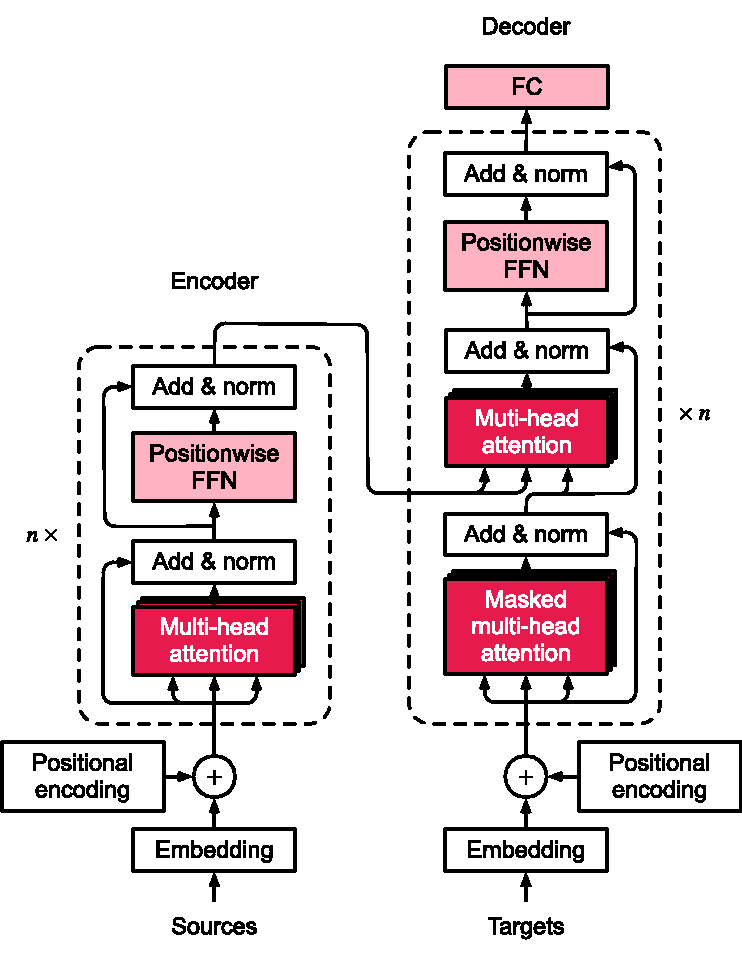
\includegraphics[width=.5\textwidth]{media/transformer.pdf}
    \caption{Diagrama de un transformer [extraído de \cite{TransformerAshish2017}]}
    \label{fig:transformer}
\end{figure}

\subsubsection{Atención}
Uno de los principales conceptos que añade el transformer es de la \textbf{atención}. Este concepto trata de emular el concepto de atención con el que todos estamos familiarizados: el de ponderar y distrubir los recursos cognitivos de forma que aquellos estímulos más importantes reciban más recursos de cómputo por parte del sistema, de la misma forma que nuestro cerebro procesa de forma más potente aquello en lo que estamos concentrados, ignorando aquellos estímulos que sean menos importantes en un determinado instante.

Uno de los principales problemas de las redes neuronales recurrentes clásicas es la imposibilidad de la paralelización de su ejecución, y el crecimiento de los términos a considerar conforme más avanzado es el análisis de la secuencia en concreto.

La técnica de \textit{multi-head attention}, que podemos apreciar en color en la Figura \ref{fig:transformer}, soluciona estos problemas. En primer lugar, hace la paralelización del modelo no solo posible, sino también muy fácil. Cada módulo calcula por separado la atención que le corresponda y posteriormente se concatenan y se transforman linealmente en la salida de la dimensión que se espera. 

Por otro lado, los modelos tradicionales sufren de no considerar dependencias entre elementos si estos están distantes en la secuencia. Los diferentes módulos calculan la atención en diferentes puntos de la secuencia de forma paralela. Las diferentes zonas pueden efectivamente considerar zonas muy distantes en tiempo constante, gracias a la paralelización. Esto efectivamente soluciona el problema de olvidar características importantes de puntos distantes, así como evitando tener que crear caminos de cálculo cada vez más largos conforme avanzamos en el análisis de la secuencia.


\subsection{Modelos basados en transformers}
Habiendo descrito brevemente la arquitectura de un transformer en general, veamos qué se ha desarrollado con esta nueva tecnología.

\subsubsection{BERT}
BERT son las siglas en inglés de \textit{Bidirectional Encoder Representations from Transformers}~\cite{bertDevlin2019}. Es un modelo de lenguaje generativo basado en un encoder bidireccional como su nombre indica. Este modelo fue uno de los primeros en realmente conseguir una fluidez comunicativa convincente. Su arquitectura preentrenada permite, con una sola capa extra, craer modelos para tareas en casi cualquier ámbito, como responder preguntas o inferencia del lenguaje, sin necesidad de modificar particularmente su arquitectura interna.


\subsubsection{LaMDA}
LaMDA corresponde con las siglas de \textit{Language Model for Dialogue Applications}~\cite{LaMDAGoogle2020}, un proyecto de Google que compite de forma directa con los modelos antes mencionados. Al igual que los dos proyectos anteriores, LaMDA está basado en un transformer, una arquitectura de redes neuronales creada también por Google~\cite{TransformerAshish2017}, que explicaremos en más profundidad en los siguientes capítulos. Este proyecto se creó con una aplicación en concreto: un \textit{chatbot} automático lo más natural posible, al que llamaron \textit{Meena}. Según las estadísticas de Google, Meena tiene casi el doble de capacidad de predicción e inferencia que el antiguo GPT-2, y se entrenó en 8 veces más datos. Es el buque insignia de la empresa.

\subsubsection{GPT-3 Open AI}
GPT son las siglas de \textit{Generative Pre-trained Transformer}~\cite{GPT3openAI2020} y 3 indica la versión. Este modelo trata de abarcar los problemas que otros transformers solían tener, como es la habilidad de un humano para continuar una tarea lingüística dado muy poco contexto o instrucciones. Escalando los modelos se logra mejorar significativamente la generalización del mismo y se descubre que no es necesario afinar los parámetros de los modelos, sino que esto puede corresponderse más con un problema de meta-aprendizaje.

Existen varias versiones del GPT-3, entrenadas en diferentes tamaños, desde 125 millones en la versión que denominan pequeña, hasta 175 mil millones, que es la versión que los investigadores denominan como ``GPT-3'' a secas. Jared Kaplan sugiere en \cite{kaplan2020scaling} que la función de pérdida en la etapa de validación debería corresponderse con la ley de potencia, (también conocida como el principio de Pareto) en función del tamaño de dicha red, de ahí que se probaran distintas configuraciones y tamaños.

Para nuestro proyecto, hemos escogido el modelo GPT-2, de OpenAI. Concretamente usaremos la versión pequeña, que consta de 117M de parámetros. Este modelo fue entrenado en una base de datos de texto tomada de Wikipedia, constando de más de 60GB de datos de texto. 

Utilizaremos el modelo preentrenado, que ya de por sí es capaz de hablar de forma genérica, y lo entrenaremos con nuestra base de datos para que aprenda a hablar tal y como lo haría un médico.




\chapter{Metodología}

En este capítulo ahondaremos en los conceptos más importantes que hemos de entender de cara al funcionamiento de nuestro modelo generativo, tanto en el entrenamiento como en la generación de comentarios.



\section{Datos de entrada}
En primer lugar, debemos ofrecer los datos de entrada al modelo. Estos datos están previamente formateados y unificados, como vimos en la fase de preprocesamiento.

Es importante la adición de las etiquetas \jesitt{<|BOS|>} y \jesitt{<|EOS|>}. Estas etiquetas son las siglas de \textit{begin of sentence} y \textit{end of sentence}. Son marcadores que indican el inicio y fin de una oración. Estas etiquetas son necesarias para que el modelo entienda cuál es el criterio a partir del cual empieza y acaba una oración.

\subsection{Codificación de los tokens}
Antes de pasar los datos al modelo, debemos codificarlos. Codificar significa obtener un código único en función del token que estemos considerando. La codificación es esencial para estos modelos, ya que ofrece una representación matemática de las palabras. La codificación de los tokens se efectúa mediante un diccionario preentrenado, de forma que la codificación y decodificación sean consistentes, dado un modelo determinado.

Este proceso es relativamente simple: para cada palabra que encontremos en el texto, le asociamos un índice y guardamos la entrada en un diccionario. De esta forma, cada vez que queramos que la red procese un extracto de texto, sustituimos cada término por su correspondiente número en el diccionario. De esta tarea también se suele encargar el Tokenizer. 

Como vimos en la sección \ref{sec:tokens}, estos algoritmos solo se encargan de transformar el texto en vectores, pero al ser una tarea perteneciente a la fase de preprocesamiento, las librerías suelen ofrecer esta funcionalidad de forma conjunta. Es el caso particular en \jesitt{transformers}. Esto también garantiza que el tokenizer utilizado para un determinado modelo sea el mismo de una ejecución a otra, ya que de otra forma habría problemas con la codificación.

\begin{figure}[h]
	\centering
	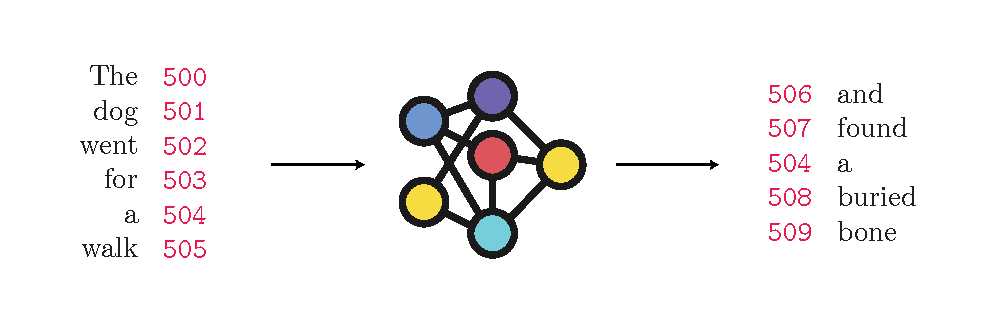
\includegraphics[width=.9\textwidth]{media/tokenizer.pdf}
	\caption{Ilustración del proceso de codificación -- decodificación necesario}
	\label{fig:codification}
\end{figure}

Una vez procesado, el modelo nos devolverá una secuencia de números, de los que podemos volver a obtener el texto subyaciente deshaciendo la operación.




\section{Ajuste de los pesos}
\begin{figure}[h]
	\centering
	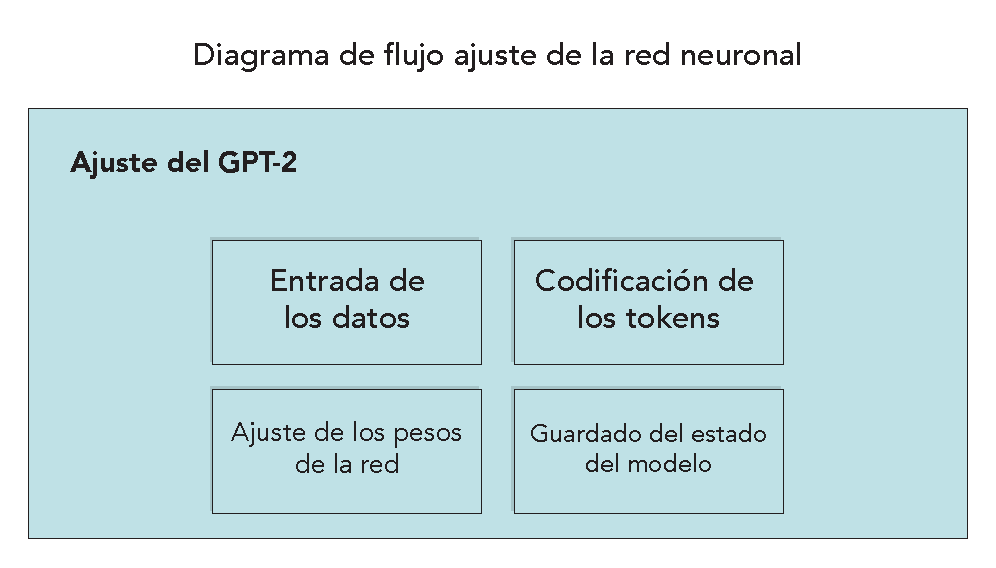
\includegraphics[width=.9\textwidth]{media/gpt-fine-tune.pdf}
	\caption{Diagrama resumen del ajuste de los pesos del GPT2}
	\label{fig:fine-tune-gpt}
\end{figure}

Nuestro modelo ya está construido. Esto es, los diseñadores ya han decidido las distintas capas y el orden de estas según hemos visto en las secciones anteriores. Este modelo se nos ofrece preentrenado de forma bastante simple. Tal y como viene en el paquete, es capaz de generar frases con relativo sentido, es decir, de algún modo \textit{sabe hablar}. 

El ajuste se efectúa como un proceso de aprendizaje no supervisado, en la que exponemos a la red a un conjunto de comentarios de forma que ésta podrá generar nuevos comentarios de la nada que caigan bajo la función de distribución de los comentarios de entrada. 

En nuestro caso, esta función de distribución la define nuestro conjunto de datos de informes médicos. Este proceso efectivamente ajusta los pesos de la red de forma que se familiarice al modelo con el vocabulario y expresiones comunes encontradas en los extractos médicos presentados.

Este proceso es, computacionalmente, extraordinariamente costoso. Debemos calcular el peso de millones de parámetros (117 millones en nuestro caso particular), debido a la magnitud del modelo. Para ello, hemos de tener disponible un equipo con, como mínimo, una tarjeta gráfica decente que nos permita hacer cálculos matriciales en paralelo, operaciones muy comunes en el entrenamiento de las redes neuronales.

Dichos equipos pueden ser muy caros. Para ello, hicimos uso del servicio de clústeres del Instituto DaSCI. En dicho servicio se nos puede asignar una máquina dependiendo de la carga que tengan las demás. Por referencia, \textbf{Selene}, uno de los equipos disponibles, consta de:
\begin{itemize}
	\item \textbf{Procesador}: Dual 20-Core Intel Xeon E5-2698 v4 2.2 GHz
	\item \textbf{RAM}: 512 GB 2,133 MHz DDR4 RAM
	\item \textbf{Disco}: 4 $\times$ 1.92 TB SSD RAID 0
	\item \textbf{Gráfica}: 8 $\times$ GPU NVIDIA Tesla V100 32GB 
\end{itemize}

Es sencillo enviar nuestros datos mediante \jesitt{ssh}, entrenamos el modelo, obtenemos los pesos y los descargamos de vuelta de la misma forma.

Gracias a \jesitt{pytorch} y \jesitt{transformers}, es también muy fácil reentrenar el GPT-2 con nuestros datos.

\subsection{Guardado del estado del modelo}
Finalmente, una vez entrenado el modelo, lo más importante es guardar su estado. Esto es muy fácil gracias a los métodos provistos por \jesitt{pytorch} y \jesitt{transformers}. Este estado se guarda en un archivo, que, generalmente, consta de un diccionario en el que las claves corresponden a los nodos de las capas en sí, es decir, a sus parámetros entrenables, y cuyo valor es el peso de dicho nodo. 

De esta forma, es fácil cargar un modelo \textit{vacío}, un modelo inicializado con pesos nulos o no relevantes, y sustituir dichos valores por los incluidos en el archivo. Esto nos permite volver al estado en el que dejamos al modelo tras el costoso entrenamiento.

\section{Generación de comentarios}

\begin{figure}[h]
	\centering
	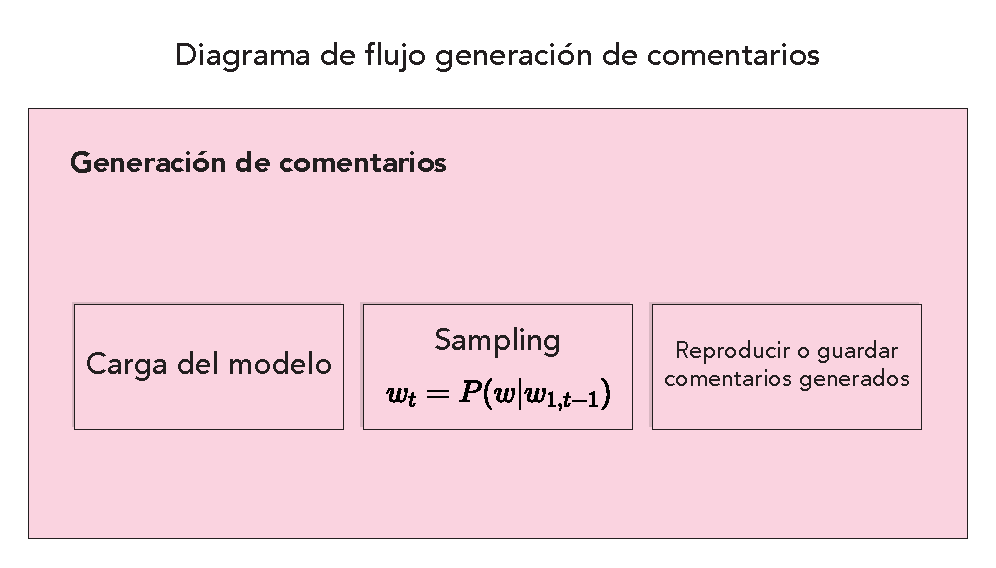
\includegraphics[width=.9\textwidth]{media/comment-gen.pdf}
	\caption{Diagrama resumen de la generación de comentarios}
	\label{fig:comment-gen}
\end{figure}

En esta sección hablaremos de la generación de comentarios, una vez nuestro modelo está entrenado y listo para funcionar. 

\subsection{Carga del modelo}
Como indicamos anteriomente, la carga del modelo es realmente sencilla gracias a las librerías que lo hacen posible. Con nuestro archivo con los pesos localizado, podemos cargar de vuelta los pesos relevantes en los parámetros correspondientes de la red, recuperando el estado original. Este estado es el que nos permitirá generar comentarios de forma automática.

\subsection{Sampling y otros métodos de generación de texto}
Una vez entrenado el modelo y ajustados los pesos, ya tenemos un marco de trabajo sobre el que poder generar comentarios de texto libre. Aun así, el modelo no es capaz de ofrecernos inferencias como en modelos clásicos de predicción o clasificación. Para poder acometer el proceso de generación de palabras, debemos efectuar una \textit{decodificación} de las mismas, y existen varias formas para acometer esto. 

Los métodos de decodificación aquí mencionados aparecen en la publicación \href{https://huggingface.co/blog/how-to-generate}{How to generate text} de Patrick von Platen. Es uno de los integrantes de Hugging Face, una de las empresa de código abierto que se dedica a la creación de los diferentes modelos mencionados anteriormente, y que nos ha provisto con una manera fácil y accesible de poder utilizar estas herramientas tan potentes con su librería \jesitt{transformers}~\cite{WolfEtal2020Transformers}.

Existen varias maneras de generar lo que en la jerga se denomina \textit{texto abierto}, es decir, generar texto de forma relativamente libre y sin restricciones. Muchos otros modelos son capaces de hacerlo, aunque nosotros nos centraremos en los métodos que conciernen a nuestro GPT2, que es un modelo autorregresivo.

Los modelos autorregresivos asumen que la siguiente palabra a generar se calcula como una función de probabilidad de todas las palabras anteriores, dada una palabra de contexto inicial. Dicho esto, existen varias maneras de \textit{decodificar} texto de un modelo de lenguaje. Veamos las más relevantes.

\subsubsection{Greedy and beam search}
La búsqueda voraz obtiene la palabra con mayor probabilidad de todas las opciones dada una palabra inicial. 


\begin{figure}[h]
	\centering

\begin{tikzpicture}
	\tikzstyle{tag}=[shape=rectangle,thick,draw,fill=white,minimum size=0.3cm]
	\tikzstyle{ntag}=[shape=rectangle,thick,draw=blue!80,fill=blue!20,minimum size=0.6cm]

	\filldraw [black] (-4,0) circle (2pt);
	
	
	%%%
	\draw (-2,0) -- node[tag] {dog} (2,3);
	\draw[red] (-2,0) -- node[tag] {nice} (2,0);
	\draw (-2,0) -- node[tag] {car} (2,-3);
	
	\node at (2, 3) [ntag, anchor= east] {0.4};
	\node at (2, 0) [ntag, anchor= east]{0.5};
	\node at (2, -3) [ntag, anchor= east]{0.1};
	
	
	%%%
	\draw[red] (2,0) -- node[tag, near start, anchor=south] {\tiny woman} (5,1);
	\draw (2,0) -- node[tag] {\tiny house} (5,0);
	\draw (2,0) -- node[tag, near start, anchor=north] {\tiny guy} (5,-1);
	
	
	
	\node at (5, 1) [ntag, anchor= east] {\tiny 0.4};
	\node at (5, 0) [ntag, anchor= east]{\tiny 0.4};
	\node at (5, -1) [ntag, anchor= east]{\tiny 0.3};
	
	%%%
	\draw (2,3) -- node[tag] {\tiny and} (5,4);
	\draw (2,3) -- node[tag] {\tiny runs} (5,3);
	\draw (2,3) -- node[tag] {\tiny has} (5,2);
	
	\node at (5, 4) [ntag, anchor= east] {\tiny 0.05};
	\node at (5, 3) [ntag, anchor= east]{\tiny 0.05};
	\node at (5, 2) [ntag, anchor= east]{\tiny 0.9};
	
	%%%
	\draw (2,-3) -- node[tag] {\tiny is} (5,-2);
	\draw (2,-3) -- node[tag] {\tiny drives} (5,-3);
	\draw (2,-3) -- node[tag] {\tiny turns} (5,-4);
	
	\node at (5, -2) [ntag, anchor= east] {\tiny 0.3};
	\node at (5, -3) [ntag, anchor= east]{\tiny 0.5};
	\node at (5, -4) [ntag, anchor= east]{\tiny 0.2};


	\draw[red] (-4,0) -- (-2,0)
	node[tag, anchor=east] {The};
\end{tikzpicture}

	\caption{Ilustración de los pasos que daría el algoritmo greedy, tomando siempre la posibilidad más alta}
	\label{tkz:greedy}
\end{figure}

Dada una palabra inicial que tomamos del usuario, por ejemplo, siempre tomaremos aquella palabra de todas las posibles opciones que más probabilidad tenga de aparecer, dada la palabra anterior. Dichas probabilidades se calculan en el entrenamiento del modelo. Podemos ver un ejemplo de este comportamiento en la Figura \ref{tkz:greedy}.

El algoritmo toma siempre la palabra más probable y esto funcionará bien, aunque este algoritmo peca de empezar a repetirse bastante pronto. Esto es, generará secuencias que contienen palabras finales e iniciales similares, por lo que el ciclo empieza de nuevo al escogerse siempre la palabra más probable.



\begin{figure}[h!]
	\centering
	
	\begin{tikzpicture}
		\tikzstyle{tag}=[shape=rectangle,thick,draw,fill=white,minimum size=0.3cm]
		\tikzstyle{ntag}=[shape=rectangle,thick,draw=blue!80,fill=blue!20,minimum size=0.6cm]
		
		
		\draw[red] (-4,0) -- (-2,0)
		node[tag, anchor=east] {The};
		
		\filldraw [black] (-4,0) circle (2pt);
		
		
		%%%
		\draw[red] (-2,0) -- node[tag] {dog} (2,3);
		\draw[red, densely dotted] (-2,0) -- node[tag] {nice} (2,0);
		\draw (-2,0) -- node[tag] {car} (2,-3);
		
		\node at (2, 3) [ntag, anchor= east] {0.4};
		\node at (2, 0) [ntag, anchor= east]{0.5};
		\node at (2, -3) [ntag, anchor= east]{0.1};
		
		
		%%%
		\draw[red, densely dotted] (2,0) -- node[tag, near start, anchor=south] {\tiny woman} (5,1);
		\draw (2,0) -- node[tag] {\tiny house} (5,0);
		\draw (2,0) -- node[tag, near start, anchor=north] {\tiny guy} (5,-1);
		
		
		
		\node at (5, 1) [ntag, anchor= east] {\tiny 0.4};
		\node at (5, 0) [ntag, anchor= east]{\tiny 0.4};
		\node at (5, -1) [ntag, anchor= east]{\tiny 0.3};
		
		%%%
		\draw (2,3) -- node[tag] {\tiny and} (5,4);
		\draw (2,3) -- node[tag] {\tiny runs} (5,3);
		\draw[red] (2,3) -- node[tag] {\tiny has} (5,2);
		
		\node at (5, 4) [ntag, anchor= east] {\tiny 0.05};
		\node at (5, 3) [ntag, anchor= east]{\tiny 0.05};
		\node at (5, 2) [ntag, anchor= east]{\tiny 0.9};
		
		%%%
		\draw (2,-3) -- node[tag] {\tiny is} (5,-2);
		\draw (2,-3) -- node[tag] {\tiny drives} (5,-3);
		\draw (2,-3) -- node[tag] {\tiny turns} (5,-4);
		
		\node at (5, -2) [ntag, anchor= east] {\tiny 0.3};
		\node at (5, -3) [ntag, anchor= east]{\tiny 0.5};
		\node at (5, -4) [ntag, anchor= east]{\tiny 0.2};
		
	
\end{tikzpicture}

	\caption{Ilustración demostrando el funcionamiento del \textit{beam search}, con 2 beams en este caso. Vemos como se toma un camino que a priori es menos probable pero resulta en una probabilidad más alta al final.}
	\label{tkz:beams}
\end{figure}


Una solución planteada es el \textit{beam search}, que podemos visualizar en la Figura \ref{tkz:beams}, algo así como una búsqueda distribuida. Dadas las probabilidades de cada palabra, el algoritmo calcula varios pasos en avanzadilla para varias alternativas, y devuelve aquella secuencia que más probabilidad general tenga. Esto soluciona algunos problemas, pero no termina de lidiar con el factor de repetitividad anterior. 

Por otro lado, Ari Holtzmann sugiere en \cite{holtzman2020curious} que la generación del lenguaje humano no se guía por la elección de las palabras más probables. El lenguaje humano real es mucho menos predecible, ya que de otra forma sería \textit{aburrido} de leer o escuchar.

Es por ello que los métodos alternativos han de evitar las técnicas \textbf{deterministas} de generación de texto, y apostar por los métodos con gran influencia aleatoria.

\subsubsection{Sampling}

Sampling es otra técnica de generación de lenguaje autorregresiva, que, como sabemos, asume la probabilidad de una palabra dada la anterior.

En la forma más básica, el muestreo simplemente toma una palabra de forma aleatoria, ponderándolas con una distribución de probabilidad tal que:

\begin{equation}
	w_t = P(w | w_{1, t-1})
\end{equation}

es decir, la probabilidad de escoger la palabra $w_t$ depende de todas las palabras anteriores.

\begin{figure}[h]
	\centering
	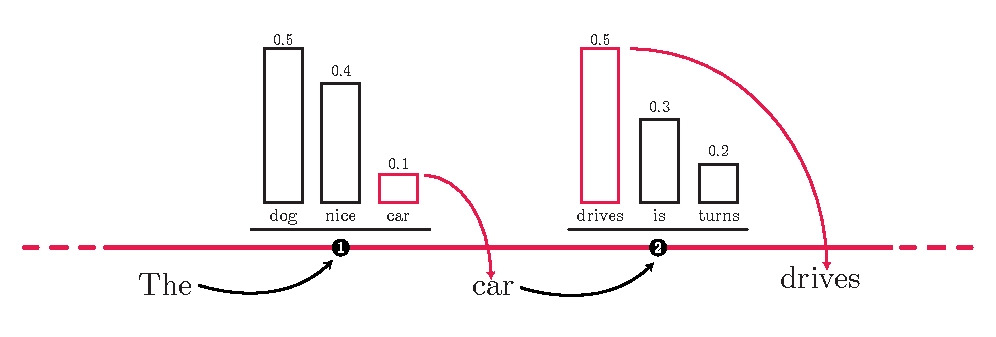
\includegraphics[width=.9\textwidth]{media/sampling.pdf}
	\caption{Ilustración de un ejemplo de muestreo. Se toman palabras aleatoriamente, aunque se pondera en función de su probabilidad.}
	\label{fig:sampling}
\end{figure}

El hecho de que una palabra presente una gran probabilidad de ser escogida no corresponde con que al final se la acabe escogiendo, como vemos en el paso 1 de la Figura \ref{fig:sampling}. En este caso, se escogió \textit{car} y posteriormente sí se escogió la palabra más probable. Este proceso nos ayuda a explorar más el espacio de búsqueda subyacente compuesto de todas las combinaciones de palabras posibles.

\subsubsection{Temperatura}
Podemos graduar la ponderación de la que hablamos con lo que los autores denominan la \textit{temperatura} de la función de activación \textit{softmax} de la última capa del modelo.

Al bajar la temperatura por debajo de 1 (siendo 1 un ajuste nulo), las palabras más probables se saturan, es decir, se hacen más probables, y las menos probables se comprimen, haciéndolas menos probables. En el otro extremo, al ajustar la temperatura a límites muy cercanos a 0, nos encontraríamos con la búsqueda voraz de la que hablamos antes.

Este factor nos ofrece una especie de regulador entre \textbf{máximo determinista} o \textbf{máximo aleatorio}.

La adición de esta técnica ayuda a que la generación no sea \textit{extremadamente} aleatoria. Si bien en la sección anterior comentábamos que debíamos añadir aleatoriedad, todo en exceso es malo. Una generación completamente aleatoria es, en su mayoría, poco coherente. La bajada sutil de la temperatura del modelo provoca que se elijan, normalmente, palabras bastante probables, pero que de vez en cuando se escojan palabras poco probables. Dichas palabras ahora abren nuevos caminos por los que continuar generando, que no hubieran sido considerados de otra forma, pero continuamos eligiendo, por lo general, combinaciones de palabras más probables, para garantizar la coherencia del texto.

En esencia, el proceso es un gran compromiso entre coherencia y predecibilidad, además de los demás grandes problemas presentes como los bucles infinitos.

\subsubsection{Top K Sampling}

Dadas las premisas anteriores, las siguientes técnicas son mejoras incrementales que tratan de solucionar algunos otros problemas existentes.

El muestreo de los K mejores, tal y como su nombre indica, solo considera las K mejores opciones de toda la batería de palabras posibles. Dado este subconjunto K, se muestrea una palabra como en el Sampling original, tomándola aleatoriamente de forma ponderada. Puede verse claramente en la Figura \ref{fig:top-k} 


\begin{figure}[h]
	\centering
	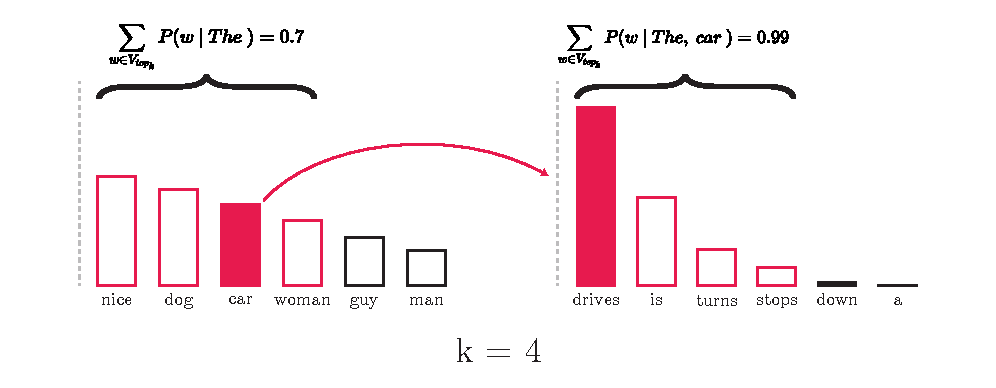
\includegraphics[width=.9\textwidth]{media/top k.pdf}
	\caption{Ilustración del proceso de cálculo en muestreo con un valor de $k = 4$.}
	\label{fig:top-k}
\end{figure}

Esta técnica elimina posibles elecciones bastante malas, lo que Holtzmann denomina como "\textit{the unreliable tail}", que podemos acuñar como \textit{la cola traicionera}, fácilmente apreciable en la ilustración. Holtzmann afirma que existe una enorme cantidad de palabras con muy baja probabilidad en cada elección que, en realidad, están sobrerepresentadas cuando hablamos de términos agregados. Es decir, la \textbf{probabilidad agregada} de todas esas palabras con una bajísima probabilidad puede corresponder a \textbf{grandes proporciones de la distribución de probabilidad}, lo que, efectivamente, va en contra de nuestro objetivo.

Tomando solo aquellas K mejores, se elimina dicha cola y se redistribuye la probabilidad de los términos elegidos de forma oportuna, creando un modelo de decodificación mucho más natural que los otros.

\subsubsection{Top P nucleus}

Finalmente, esta última técnica se denomina Top P nucleus, refiriéndose a un valor diferente al K anterior.

En este caso, en lugar de tomar los K mejores términos, tomamos el conjunto más pequeño de términos cuya probabilidad acumulada supere el $p$ establecido por el usuario. Esto es, dado un $p = 0.9$, tomamos las $n$ mejores palabras que, dada la suma de su probabilidad, se supere el $p$ determinado. El proceso es básicamente idéntico al ilustrado en la Figura \ref{fig:top-k}, solo que consideramos la probabilidad acumulada, no un número de términos.

Esto provoca que en lugar de tomar un subconjunto de palabras de cardinalidad constante durante todo el proceso, ahora el tamaño varía. Se ha demostrado que esta flexibilidad ayuda y contribuye a una generación de texto más natural.

Estos dos últimos métodos son los más utilizados en el estado del arte, y este último es el que \textbf{utilizamos nosotros} en nuestro proyecto a la hora de generar palabras. Como vemos, aun disponiendo de una red neuronal muy potente, no es trivial extraer información coherente y de calidad.
\chapter{Experimentación: modelos \\ y entrenamiento}

En este capítulo usaremos todos los conceptos vistos en los capítulos anteriores para justificar las elecciones de los diferentes modelos, hablaremos de las características principales de los mismos y finalmente entraremos en la fase del entrenamiento y los resultados de dichos modelos.







\section{Experimentación}


\section{Resultados}
\chapter{Análisis de textos médicos}

En este capítulo discutiremos cómo hemos llevado a cabo la evaluación de las herramientas disponibles en el estado del arte para la extracción de información en texto no estructurado de carácter médico.

Para ello se ha creado una web app disponible de forma muy accesible para que sea fácil ver el poder combinado de todas estas herramientas. Dicha herramienta se denomina \href{https://share.streamlit.io/jesi-rgb/medical-text-analysis/src/streamlit_gen_test.py}{MEDGEN}.



\section{Despliegue de MEDGEN}

Para hacer accesible todo el trabajo que se ha acometido, se ha elaborado una aplicación que permite hacer uso de todas las técnicas y herramientas discutidas a lo largo del documento. 

El framework utilizado ha sido \href{https://streamlit.io}{Streamlit}. Streamlit es un framework para Python diseñado para el prototipado ágil de aplicaciones web. Los creadores idearon esta herramienta para disminuir el esfuerzo que hay que acometer a la hora de desplegar una aplicación basada en inteligencia artificial, es decir, una aplicación que consta de sistemas de inferencia o similares, sistemas que no se encuentran en aplicaciones web usuales. 

De esta forma, es muy accesible y sencillo diseñar una aplicación en Python, donde se puede integrar cualquier sistema de IA en desarrollo y habilitar un espacio para que personas ajenas al desarrollo experimenten de primera mano cómo funciona, ofreciendo la oportunidad de crear casos de uso reales.

La aplicación permite generar comentarios utilizando el modelo generativo, y permite analizar dichos comentarios, así como importar desde distintas fuentes. La aplicación efectúa un pequeño análisis del texto y utiliza el tagger que el usuario seleccione.

\section{Evaluación de las herramientas}

Como vemos en las Figuras \ref{fig:app-demo} y \ref{fig:analysis-comment}, podemos efectuar nuestro análisis de diferentes formas. La aplicación nos permite utilizar los NER Taggers indicados en la Sección \ref{sec:nertagger}: Med7, BC5CDR y BIONLP13CG.

Podemos, en caso de no disponer de un conjunto de datos, generar comentarios usando nuestro modelo generativo. Una vez generados, podemos analizarlos con el NER Tagger que deseemos. Aquí, el desarrollador estaría programando el suyo propio y podría integrarlo al sistema fácilmente para testearlo de forma apropiada. 

El análisis nos ofrece una versión etiquetada del texto original, así como unas estadísticas del comentario en concreto. Además de ello, podemos importar nuestros propios comentarios desde un archivo o copiarlos y pegarlos en el campo de texto, con tal de maximizar la comodidad de uso de la aplicación.

En función del texto de entrada y el Tagger seleccionado obtendremos mejores o peores resultados. El generador de comentarios está entrenado para generar comentarios de carácter quirúrgico o post-operatorios. Para ello, el BIONLP13CG es una buena elección, pero el Med7 rara vez será capaz de ofrecer resultados, ya que está especializado en recetas médicas.

La ventaja de esto es el gran abanico de posibilidades que tenemos de forma muy accesible, siendo posible analizar casi cualquier tipo de texto médico que sea de interés. De no disponer de un Tagger apropiado, siempre podemos incluirlo en la aplicación, como mencionábamos en la Sección \ref{sec:nertagger}.

\begin{figure}[h]
	\centering
	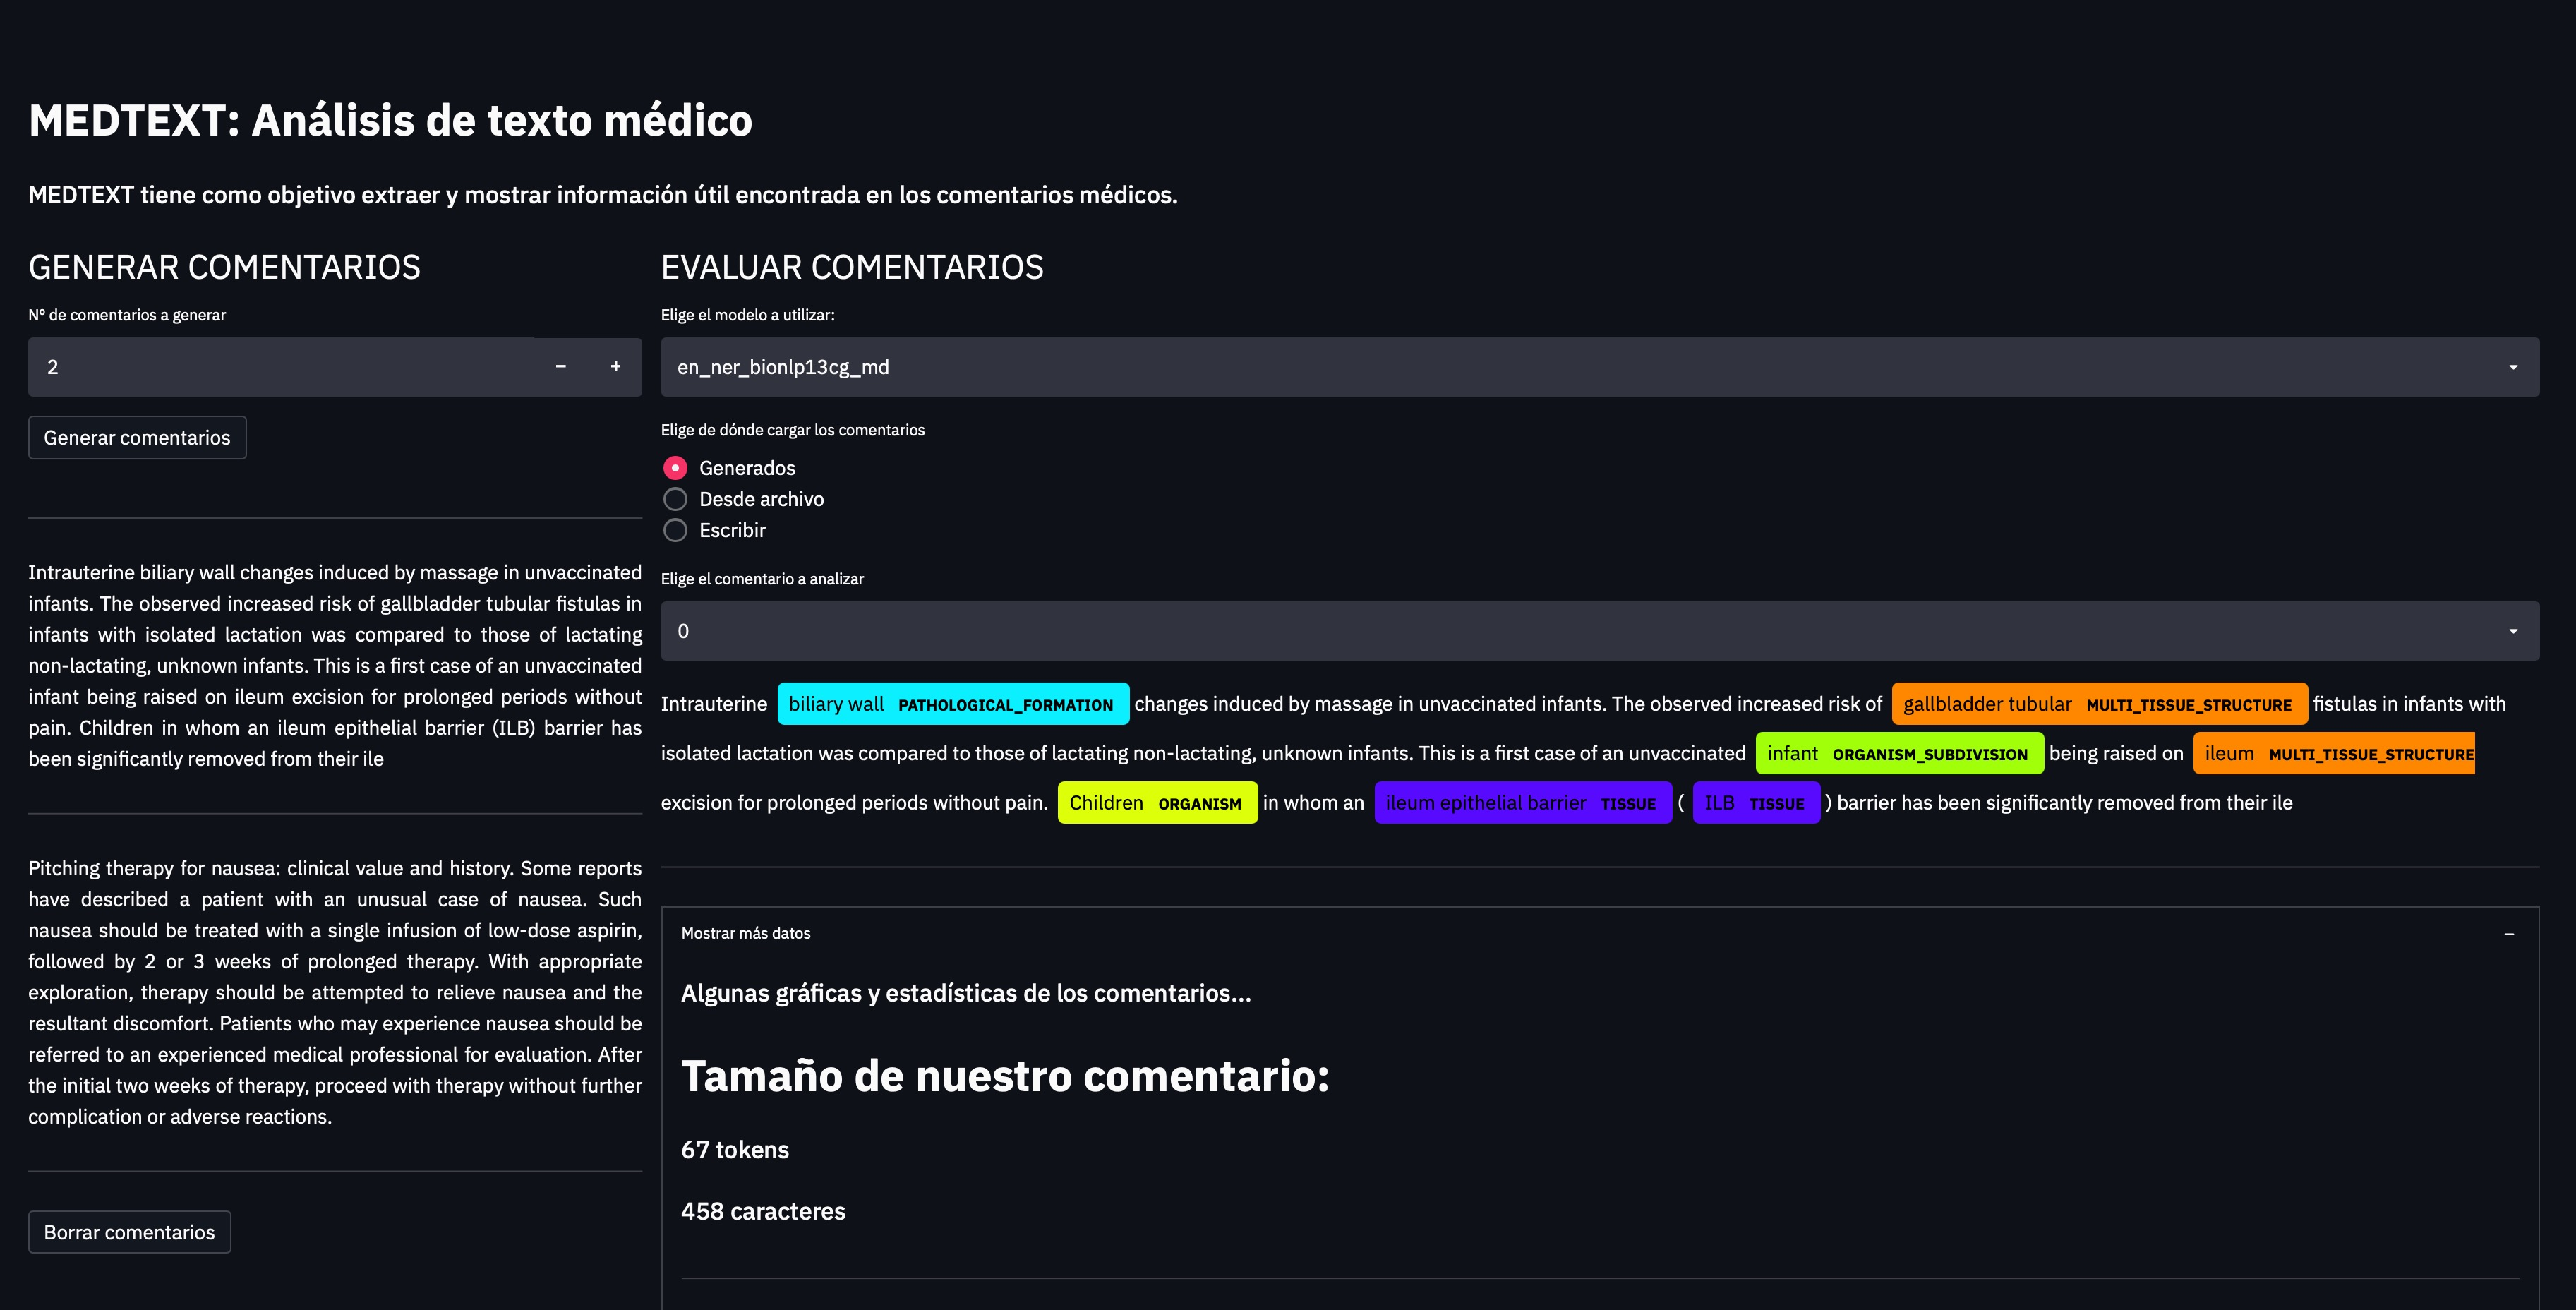
\includegraphics[width=.9\textwidth]{media/app_demo.jpeg}
	\caption{Captura de pantalla de la aplicación elaborada. A la izquierda podemos generar comentarios y a la derecha, analizarlos.}
	\label{fig:app-demo}
\end{figure}


\begin{figure}[h]
	\centering
	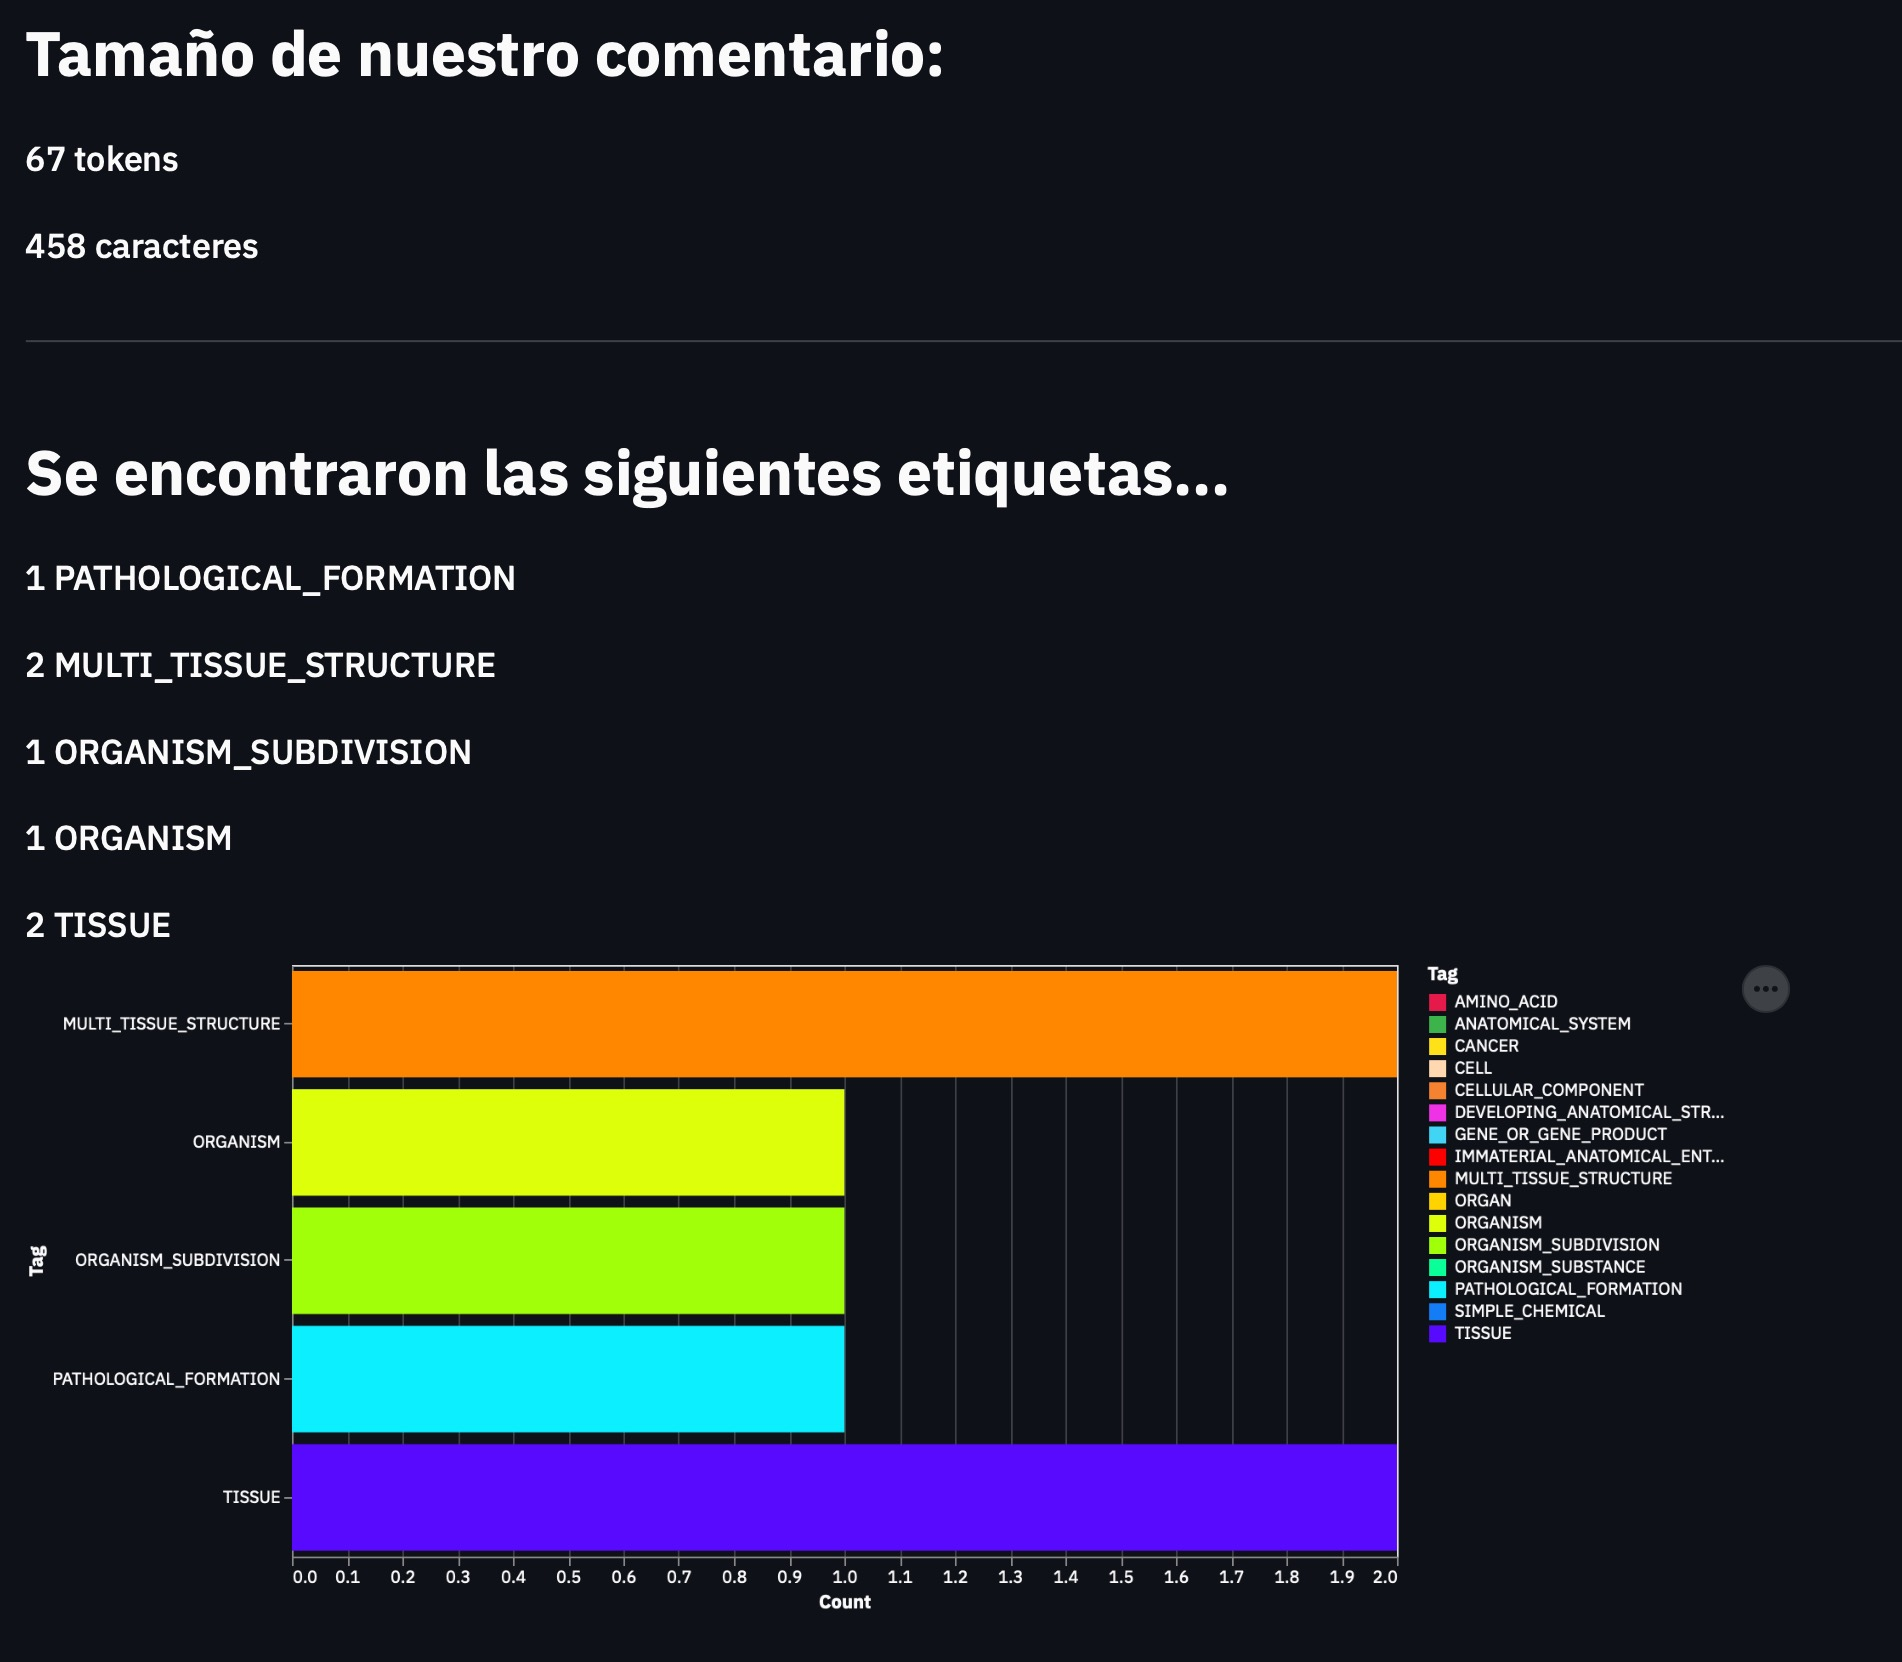
\includegraphics[width=.62\textwidth]{media/analysis_comment.jpeg}
	\caption{Captura de pantalla del análisis que ofrece la aplicación acerca de un determinado comentario.}
	\label{fig:analysis-comment}
\end{figure}



\section{Instalación y modo de uso}
La aplicación puede compilarse desde el código fuente siguiendo el \href{https://github.com/jesi-rgb/medical-text-analysis}{enlace al repositorio}, descargándolo y ejecutando los siguientes comandos:

\jesitt{git clone https://github.com/jesi-rgb/medical-text-analysis}

Activamos el entorno que más nos guste, ya sea de python o conda.

\jesitt{cd medical-text-analysis}

\jesitt{pip install -r requirements.txt}

Una vez finalizado, 

\jesitt{streamlit run src/streamlit\_gen\_test.py}

se nos abrirá una ventana en el navegador y la aplicación estará lista para funcionar.

La primera ejecución tarda un poco más, ya que ha de descargar el modelo de Internet y cargarlo en memoria. Tras eso, los modelos se guardan en caché y la ejecución es mucho más rápida.

\chapter{Conclusiones}
En este último capítulo abordaremos todos los problemas y objetivos propuestos a lo largo de este proyecto con objeto de refrescarlos, y finalmente se ofrecerá una evaluación acerca de cómo estos objetivos se han cumplido. Finalmente se reflexionará acerca de cómo podría extrapolarse este proyecto de cara al futuro.

\section{Problemática inicial}
Para empezar, hablaremos del problema inicial que nos ha motivado en la elaboración de esta herramienta.

Los informes médicos ofrecen grandes cantidades de información clave para los profesionales de cara al tratamiento de los pacientes, y gran parte de esta información se almacena en cuerpos de texto libre. Dichos extractos usualmente no se utilizan de cara a la extracción de información automática debido a la naturaleza no estructurada de los mismos, que hace su análisis muy complicado.

Aún así, en estas secciones se puede encontrar mucha información muy valiosa y relevante, por lo que tratar de encontrar un sistema automático que pueda ofrecer información estructurada dado un conjunto de información no estructurada puede ser de gran utilidad en el ámbito médico profesional.

\section{Objetivos propuestos}
Dada la problemática inicial, el objetivo es crear una herramienta que pueda ofrecer información estructurada. Una de las herramientas más útiles en este caso es un reconocedor de entidades, o, en inglés, un NER Tagger. Dado un texto, es capaz de reconocer entidades importantes automáticamente.

En el contexto médico, debemos atender a las entidades más importantes como los medicamentos, enfermedades, partes del cuerpo, etc. Para ello, existe un vocabulario unificado, denomidando SNOMED. Gracias a esto, podemos averiguar con precisión dónde se hallan los datos más importantes.

Si bien se han creado varios reconocedores de entidades, cada uno construido para diferentes tareas dentro del ámbito médico (desde recetas de medicamentos hasta informes quirúrjicos), se pretendía crear un sistema con el que el desarrollo de nuevos reconocedores fuera más fácil. Esto implica disponer de ingentes cantidades de datos que, por su delicada corte, pueden no estar fácilmente disponibles.

Es por ello, que en pos de alcanzar este primer objetivo de facilitar el desarrollo de reconocedores de entidades (o cualquier otro tipo de herramienta relacionada), se plantea un segundo objetivo: un generador de comentarios automático.

Un generador de comentarios automático elimina la necesidad de inspeccionar en busca de conjuntos de datos, ya que se podrán generar cuantos se deseen, de cara al desarrollo de las herramientas. Esto es además viable gracias al destacable avance acometido en los campos de inteligencia artificial, donde se han creado modelos de lenguaje muy competentes.


\section{Metogología y resultados}
Es por ello que disponemos de dos objetivos: 
\begin{enumerate}
	\item Crear un modelo de lenguaje generativo que sea capaz de generar comentarios de forma automática.
	\item Disponiendo de un conjunto de datos \textit{infinito}, habilitar un sencillo desarrollo de herramientas de extracción de conocimiento de texto.
\end{enumerate}

Para ello, se han utilizado modelos generativos de lenguaje preentrenados, como el GPT-2. El GPT-2 es un \textit{transformer}, un tipo de arquitectura de red neuronal especializada en procesamiento de texto de forma paralela. El GPT-2 es un modelo preentrenado y abierto, lo que nos habilita a poder crear una herramienta que genere comentarios de forma automática.

Se ha observado que el modelo es capaz de crear comentarios de forma bastante competente con un entrenamiento previo en un conjunto de datos preprocesado y unificado manualmente, lo que los creadores denominan como \textit{fine-tuning} de la red. 

Esto hace el desarrollo de dichos modelos más fácil para todos, contribuyendo a una mayor y mejor producción de herramientas de asistencia médica, clave para cualquier complejo hospitalario medianamente grande, donde se manejan volúmenes de datos, a menudo, insostenibles.

La asistencia que estas herramientas ofrecen puede suponer una mejora en la calidad de la atención que cada paciente recibe, además de la reducción de carga cognitiva que los correspondientes profesionales deben soportar, mejorando la calidad de vida de ambas partes. Con todo ello, se apunta a una mejora del sistema médico del que disponemos, del que ya de por sí podemos estar orgullosos siendo uno de los mejores en el mundo.

\section{Posibles trabajos futuros}

Partiendo del punto en el que nos encontramos, podemos dirigir el proyecto en varias direcciones.

Podemos centrarnos en desarrollar un sistema de reconocimiento de entidades que unifique todos los existentes y los mejore, con ayuda del SNOMED y de los datos públicos disponibles.

Por otro lado, podemos centrarnos en el ámbito de la red neuronal que hemos construido. El GPT-2 no solo puede generar comentarios, puede resumir y puede clasificar texto. Esto permite que, con la correcta configuración, obtengamos, por ejemplo, un resumen de un informe médico de forma que no tengamos que leer todo el contenido para obtener toda la información.

Con ayuda del clasificador, se puede crear un sistema de recomendación y búsqueda para una base de datos muy poderoso. Buscando términos relativamente ambiguos, tal y como un humano preguntaría de forma natural, el sistema es capaz de devolver todos aquellos documentos relacionados, de forma que el acceso a los documentos en la base de datos es ahora mucho más fácil y natural.












\appendix
\chapter{First Appendix}








\bibliographystyle{unsrt}
\bibliography{bibs/bibliography}
\addcontentsline{toc}{chapter}{Bibliografía}

\end{document}